\begin{surferPage}[99 singulariteter]{En flate av sjuende grad med 99 singulariteter}
	Oliver Labs konstruerte en flate av sjuende grad mens han jobbet med avhandlingen sin 
	ved Universitetet i Mainz i 2004. Dette er den foreløpige verdensrekorden for en flate av sjuende 
	grad, men det kan fortsatt finnes en slik flate med opptil $104$ singulariteter! Flaten til Labs har 
	symmetrien til et vanlig heptagon (bildet til venstre). Det blir synlig når vi ser på flaten ovenfra (bildet til høyre):
	
    \vspace*{-0.3em}
    \begin{center}
      \begin{tabular}{c@{\qquad}c}
        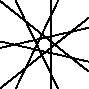
\includegraphics[height=1.5cm]{./../../common/images/labsseptic1.pdf}
        &
        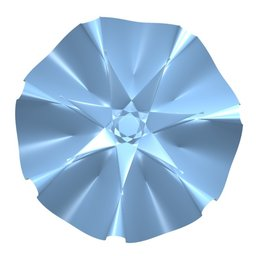
\includegraphics[height=1.5cm]{./../../common/images/labs_septic_von_oben}
      \end{tabular}
    \end{center}
    \vspace*{-0.3em}
	
	For å konstruere denne flaten, brukte Oliver Labs det algebraiske dataprogrammet {\sc Singular} 
	(Universitetet i Kaiserslautern). Det er velegnet til beregninger innen algebraisk geometri og singulariteter. 

	Labs brukte det faktum at man kan gjøre beregninger i endelige tallsystemer, som er systemer der tallene begynner 
	på nytt når de kommer til enden. Vi kjenner til dette fra klokken; 24.00$=$0.00, 24.00 $+$ 1 time er ikke 25.00, men 1.00.
\end{surferPage}
